\section{Réfraction}
Le calcul du rayon réfracté est un peu plus compliqué :
\begin{center}
\inputcode[bgcolor=bg]{c++}{code/refraction.cc}
\end{center}

D'un part, il faut déterminer si le rayon est entrant ou sortant. Pour cela,
je compare la direction de la normale avec le rayon incident. Si les deux
rayons sont de même sens alors le rayon est entrant.\footnote{Pour se
convaincre du calcul de \ttt{input}, un simple dessin suffit.} Sinon il est
sortant.

Avant de calculer le rayon réfracté, nous devons vérifier que l'angle entre
la normal et le rayon incident ne dépasse pas l'angle maximale de réfraction.
Autrement dit, si le rayon est rasant, il y a réflexion totale.

Enfin, le calcul du rayon absorbé est fait selon la loi de Snell-Descartes :
$$n_1.\sin(\theta_1) = n_2.\sin(\theta_2)$$

\subsection{Exemple}
\begin{figure}[h]
  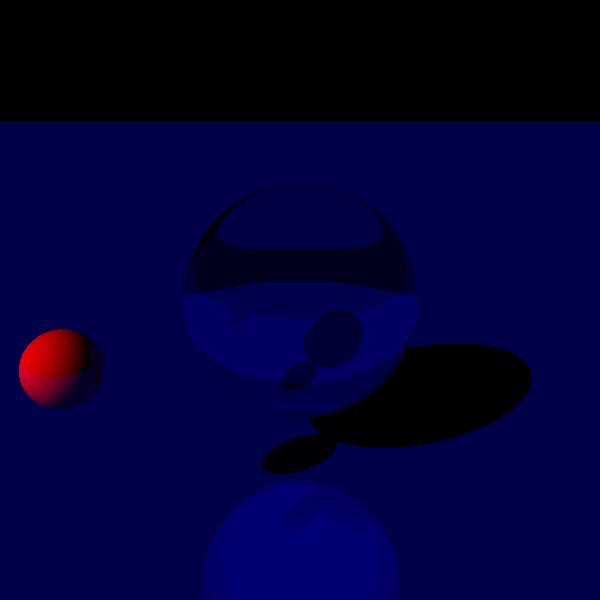
\includegraphics[width=\textwidth, keepaspectratio=true]{../../diary/09.png}
  \caption{Un exemple du rendu de la réfraction de l'environnement sur une
  sphere}
\end{figure}

\subsection{Amélioration \& bug connu}
Aucun.
